% Ara Rapor (TR) — IEEE Conference Template (IEEEtran V1.8b, conference_101719.tex yapısı)
% Derleme: pdflatex -> bibtex -> pdflatex x2.  Sayılar ../numbers.tex (src/make_macros.py) dosyasından gelir.
\documentclass[conference]{IEEEtran}
\IEEEoverridecommandlockouts
\usepackage[T1]{fontenc}
\usepackage[utf8]{inputenc}
\usepackage{babel}
\babelprovide[import,main]{turkish}
\usepackage{cite}
\usepackage{amsmath,amssymb,amsfonts}
\usepackage{graphicx}
\usepackage{textcomp}
\usepackage{xcolor}
\usepackage{booktabs,tabularx}
\usepackage[hidelinks]{hyperref}
\usepackage{xurl}
\usepackage{enumitem}
\setlist{nosep,leftmargin=*}
% OTOMATİK ÜRETİLDİ: src/make_macros.py
\newcommand{\GnegTr}{28.76}
\newcommand{\GnegTrTR}{28{,}76}
\newcommand{\GnegTe}{29.24}
\newcommand{\GnegTeTR}{29{,}24}
\newcommand{\GminTr}{-28{,}400}
\newcommand{\GminTrTR}{-28.400}
\newcommand{\GmaxTr}{61{,}228}
\newcommand{\GmaxTrTR}{61.228}
\newcommand{\GminTe}{-26{,}775}
\newcommand{\GminTeTR}{-26.775}
\newcommand{\GmaxTe}{71{,}369}
\newcommand{\GmaxTeTR}{71.369}
\newcommand{\GltHundTr}{46.25}
\newcommand{\GltHundTrTR}{46{,}25}
\newcommand{\GltHundTe}{47.89}
\newcommand{\GltHundTeTR}{47{,}89}
\newcommand{\GltTwentyTr}{32.37}
\newcommand{\GltTwentyTrTR}{32{,}37}
\newcommand{\GgtCeilTr}{0.857}
\newcommand{\GgtCeilTrTR}{0{,}857}
\newcommand{\GgtCeilTe}{0.799}
\newcommand{\GgtCeilTeTR}{0{,}799}
\newcommand{\GPpct}{28.2}
\newcommand{\GPpctTR}{28{,}2}
\newcommand{\GApct}{70.2}
\newcommand{\GApctTR}{70{,}2}
\newcommand{\GMpct}{1.6}
\newcommand{\GMpctTR}{1{,}6}
\newcommand{\GlogNegInf}{1{,}615}
\newcommand{\GlogNegInfTR}{1.615}
\newcommand{\GlogNaN}{147{,}174}
\newcommand{\GlogNaNTR}{147.174}
\newcommand{\GlogBad}{28.99}
\newcommand{\GlogBadTR}{28{,}99}
\newcommand{\GneverP}{1{,}971}
\newcommand{\GneverPTR}{1.971}
\newcommand{\GallP}{329}
\newcommand{\GallPTR}{329}
\newcommand{\GPminS}{19.1}
\newcommand{\GPminSTR}{19{,}1}
\newcommand{\GPmaxS}{40.5}
\newcommand{\GPmaxSTR}{40{,}5}
\newcommand{\GnegA}{99.28}
\newcommand{\GnegATR}{99{,}28}
\newcommand{\GrobustZ}{0.80}
\newcommand{\GrobustZTR}{0{,}80}
\newcommand{\GiqrOut}{4.53}
\newcommand{\GiqrOutTR}{4{,}53}
\newcommand{\GiqrGenes}{60.0}
\newcommand{\GiqrGenesTR}{60{,}0}
\newcommand{\GiqrPat}{64}
\newcommand{\GiqrPatTR}{64}
\newcommand{\GiqrPatPct}{10.55}
\newcommand{\GiqrPatPctTR}{10{,}55}
\newcommand{\GoutPat}{64}
\newcommand{\GoutPatTR}{64}
\newcommand{\GoutPct}{1.56}
\newcommand{\GoutPctTR}{1{,}56}
\newcommand{\GmisPos}{14}
\newcommand{\GmisPosTR}{14}
\newcommand{\GfiltAll}{3{,}571}
\newcommand{\GfiltAllTR}{3.571}
\newcommand{\GfiltTwenty}{3{,}859}
\newcommand{\GfiltTwentyTR}{3.859}
\newcommand{\GfiltTr}{3{,}051}
\newcommand{\GfiltTrTR}{3.051}
\newcommand{\GskewRaw}{1.16}
\newcommand{\GskewRawTR}{1{,}16}
\newcommand{\GskewLog}{0.05}
\newcommand{\GskewLogTR}{0{,}05}
\newcommand{\GbelowClip}{47}
\newcommand{\GbelowClipTR}{47}
\newcommand{\GpcA}{16.1}
\newcommand{\GpcATR}{16{,}1}
\newcommand{\GpcB}{11.4}
\newcommand{\GpcBTR}{11{,}4}
\newcommand{\GpcC}{6.0}
\newcommand{\GpcCTR}{6{,}0}
\newcommand{\GpcTen}{54.4}
\newcommand{\GpcTenTR}{54{,}4}
\newcommand{\GpcEighty}{34}
\newcommand{\GpcEightyTR}{34}
\newcommand{\GpcAclass}{0.30}
\newcommand{\GpcAclassTR}{0{,}30}
\newcommand{\GpcAset}{0.005}
\newcommand{\GpcAsetTR}{0{,}005}
\newcommand{\GpcBclass}{5.7\times10^{-8}}
\newcommand{\GpcBclassTR}{5{,}7\times10^{-8}}
\newcommand{\GpcBset}{0.70}
\newcommand{\GpcBsetTR}{0{,}70}
\newcommand{\GpcAsource}{0.08}
\newcommand{\GpcAsourceTR}{0{,}08}
\newcommand{\GpcAbmpb}{0.95}
\newcommand{\GpcAbmpbTR}{0{,}95}
\newcommand{\GsilClass}{0.140}
\newcommand{\GsilClassTR}{0{,}140}
\newcommand{\GsilSet}{0.049}
\newcommand{\GsilSetTR}{0{,}049}
\newcommand{\GdeFive}{608}
\newcommand{\GdeFiveTR}{608}
\newcommand{\GdeOne}{270}
\newcommand{\GdeOneTR}{270}
\newcommand{\GdeMWU}{540}
\newcommand{\GdeMWUTR}{540}
\newcommand{\GdeLfc}{313}
\newcommand{\GdeLfcTR}{313}
\newcommand{\GdeUpAML}{273}
\newcommand{\GdeUpAMLTR}{273}
\newcommand{\GdeUpALL}{335}
\newcommand{\GdeUpALLTR}{335}
\newcommand{\GlfcR}{0.70}
\newcommand{\GlfcRTR}{0{,}70}
\newcommand{\GsignAgree}{100}
\newcommand{\GsignAgreeTR}{100}
\newcommand{\GtopTest}{44}
\newcommand{\GtopTestTR}{44}
\newcommand{\GmedSetP}{0.015}
\newcommand{\GmedSetPTR}{0{,}015}
\newcommand{\GiqrSetP}{0.474}
\newcommand{\GiqrSetPTR}{0{,}474}
\newcommand{\GPcallSetP}{0.07}
\newcommand{\GPcallSetPTR}{0{,}07}
\newcommand{\GksALL}{32}
\newcommand{\GksALLTR}{32}
\newcommand{\GksAML}{0}
\newcommand{\GksAMLTR}{0}
\newcommand{\GksALLp}{17.5}
\newcommand{\GksALLpTR}{17{,}5}
\newcommand{\GksAMLp}{7.9}
\newcommand{\GksAMLpTR}{7{,}9}
\newcommand{\Gaffx}{19}
\newcommand{\GaffxTR}{19}
\newcommand{\GmisClust}{12, 25, 67}
\newcommand{\GmisN}{3}
\newcommand{\GmisNTR}{3}
\newcommand{\GtePB}{10}
\newcommand{\GtePBTR}{10}
\newcommand{\GteSJ}{8}
\newcommand{\GteSJTR}{8}
\newcommand{\GteCCG}{5}
\newcommand{\GteCCGTR}{5}
\newcommand{\GteCALGB}{4}
\newcommand{\GteCALGBTR}{4}
\newcommand{\GteDFCI}{17}
\newcommand{\GteDFCITR}{17}
\newcommand{\GallT}{9}
\newcommand{\GallTTR}{9}
\newcommand{\GallB}{38}
\newcommand{\GallBTR}{38}
\newcommand{\Sn}{1{,}292}
\newcommand{\SnTR}{1.292}
\newcommand{\Sp}{54{,}630}
\newcommand{\SpTR}{54.630}
\newcommand{\SnALL}{750}
\newcommand{\SnALLTR}{750}
\newcommand{\SnAML}{542}
\newcommand{\SnAMLTR}{542}
\newcommand{\Stotal}{2{,}096}
\newcommand{\StotalTR}{2.096}
\newcommand{\Snsub}{14}
\newcommand{\SnsubTR}{14}
\newcommand{\SallPct}{58.0}
\newcommand{\SallPctTR}{58{,}0}
\newcommand{\SamlPct}{42.0}
\newcommand{\SamlPctTR}{42{,}0}
\newcommand{\Snan}{0}
\newcommand{\SnanTR}{0}
\newcommand{\Smin}{0.00}
\newcommand{\SminTR}{0{,}00}
\newcommand{\Smax}{1.00}
\newcommand{\SmaxTR}{1{,}00}
\newcommand{\Smedian}{0.25}
\newcommand{\SmedianTR}{0{,}25}
\newcommand{\Sneg}{0.320}
\newcommand{\SnegTR}{0{,}320}
\newcommand{\SoutMed}{12}
\newcommand{\SoutMedTR}{12}
\newcommand{\SoutIqr}{372}
\newcommand{\SoutIqrTR}{372}
\newcommand{\SoutCor}{19}
\newcommand{\SoutCorTR}{19}
\newcommand{\SoutAny}{391}
\newcommand{\SoutAnyTR}{391}
\newcommand{\Sexpr}{51{,}287}
\newcommand{\SexprTR}{51.287}
\newcommand{\Siqr}{30}
\newcommand{\SiqrTR}{30}
\newcommand{\Sskew}{0.23}
\newcommand{\SskewTR}{0{,}23}
\newcommand{\SpcA}{17.6}
\newcommand{\SpcATR}{17{,}6}
\newcommand{\SpcB}{6.9}
\newcommand{\SpcBTR}{6{,}9}
\newcommand{\SpcAclass}{1.0\times10^{-300}}
\newcommand{\SpcAclassTR}{1{,}0\times10^{-300}}
\newcommand{\SsilClass}{0.490}
\newcommand{\SsilClassTR}{0{,}490}
\newcommand{\SdeFive}{37{,}742}
\newcommand{\SdeFiveTR}{37.742}
\newcommand{\SdeLfc}{0}
\newcommand{\SdeLfcTR}{0}
\newcommand{\ScommonG}{5{,}493}
\newcommand{\ScommonGTR}{5.493}
\newcommand{\SgolubG}{5{,}545}
\newcommand{\SgolubGTR}{5.545}
\newcommand{\SgseG}{22{,}880}
\newcommand{\SgseGTR}{22.880}
\newcommand{\SlfcR}{0.60}
\newcommand{\SlfcRTR}{0{,}60}
\newcommand{\SlfcRho}{0.49}
\newcommand{\SlfcRhoTR}{0{,}49}
\newcommand{\SovFifty}{14}
\newcommand{\SovFiftyTR}{14}
\newcommand{\SovHund}{34}
\newcommand{\SovHundTR}{34}
\newcommand{\SovHundExp}{1.82}
\newcommand{\SovHundExpTR}{1{,}82}
\newcommand{\SovHundP}{3.5\times10^{-36}}
\newcommand{\SovHundPTR}{3{,}5\times10^{-36}}
\newcommand{\SovTwoH}{74}
\newcommand{\SovTwoHTR}{74}
\newcommand{\SmedG}{7.27}
\newcommand{\SmedGTR}{7{,}27}
\newcommand{\SmedS}{0.42}
\newcommand{\SmedSTR}{0{,}42}
\newcommand{\SiqrG}{2.33}
\newcommand{\SiqrGTR}{2{,}33}
\newcommand{\SiqrS}{0.40}
\newcommand{\SiqrSTR}{0{,}40}
\newcommand{\SmeanRho}{0.54}
\newcommand{\SmeanRhoTR}{0{,}54}
\newcommand{\SsortDiff}{0.0059}
\newcommand{\SsortDiffTR}{0{,}0059}
\newcommand{\SaffxDrop}{45}
\newcommand{\SaffxDropTR}{45}
\newcommand{\ScorMin}{0.202}
\newcommand{\ScorMinTR}{0{,}202}
\newcommand{\ScorMed}{0.365}
\newcommand{\ScorMedTR}{0{,}365}
\newcommand{\SbmALL}{710}
\newcommand{\SbmALLTR}{710}
\newcommand{\SpbALL}{40}
\newcommand{\SpbALLTR}{40}
\newcommand{\SbmAML}{501}
\newcommand{\SbmAMLTR}{501}
\newcommand{\SpbAML}{41}
\newcommand{\SpbAMLTR}{41}
\newcommand{\SbmN}{1{,}211}
\newcommand{\SbmNTR}{1.211}
\newcommand{\SpbN}{81}
\newcommand{\SpbNTR}{81}
\newcommand{\SpcBclass}{1.3\times10^{-5}}
\newcommand{\SpcBclassTR}{1{,}3\times10^{-5}}
\newcommand{\SpcAtissue}{0.010}
\newcommand{\SpcAtissueTR}{0{,}010}
\newcommand{\SpcBtissue}{0.25}
\newcommand{\SpcBtissueTR}{0{,}25}
\newcommand{\StisALL}{1{,}076}
\newcommand{\StisALLTR}{1.076}
\newcommand{\StisAML}{293}
\newcommand{\StisAMLTR}{293}
\newcommand{\SpcC}{6.1}
\newcommand{\SpcCTR}{6{,}1}
\newcommand{\SbetaDiff}{0.019}
\newcommand{\SbetaDiffTR}{0{,}019}
\newcommand{\SbetaMed}{0.2496}
\newcommand{\SbetaMedTR}{0{,}2496}
\newcommand{\SsilDraw}{0.993}
\newcommand{\SsilDrawTR}{0{,}993}
\newcommand{\SsilDz}{-0.177}
\newcommand{\SsilDzTR}{-0{,}177}
\newcommand{\SsilCz}{0.346}
\newcommand{\SsilCzTR}{0{,}346}
\newcommand{\SrawPCone}{98.9}
\newcommand{\SrawPConeTR}{98{,}9}
\newcommand{\SheatAgree}{97.3}
\newcommand{\SheatAgreeTR}{97{,}3}
\newcommand{\SheatMisALL}{29}
\newcommand{\SheatMisALLTR}{29}
\newcommand{\SheatMisAML}{6}
\newcommand{\SheatMisAMLTR}{6}
\newcommand{\SovGenes}{ANXA1, APLP2, BLK, CD19, CD22, CD33, CD63, CD79A, CD79B, CEBPD, CFD, CHRFAM7A}
\newcommand{\StopTen}{LEF1-AS1, PNKD, LEF1, MGST1, LEF1, MGST1}

\newcommand{\PvideoURL}{\textcolor{red}{[video URL'si eklenecek]}}
\newcommand{\PrepoURL}{\url{https://github.com/pervinncelikk/ML-ALL-AML-PROJECT}}
\graphicspath{{../../results/figures/tr/}}
\AtBeginDocument{\renewcommand{\tablename}{TABLO}\renewcommand{\abstractname}{Özet}}
\renewcommand{\IEEEkeywordsname}{Anahtar Kelimeler}
\setlength{\textfloatsep}{6pt plus 2pt minus 2pt}
\setlength{\dbltextfloatsep}{6pt plus 2pt minus 2pt}
\setlength{\abovecaptionskip}{2pt}

\begin{document}

\title{Gen İfadesi Mikrodizi Verisiyle ALL/AML Lösemi Alt Tip Sınıflandırması: Literatür, Veri Setleri ve Keşifsel Veri Analizi\\
{\large Makine Öğrenmesi Dersi Dönem Projesi --- Ara Rapor}}

\author{\IEEEauthorblockN{Pervin Çelik \quad (Öğrenci No: 503020250010)}
\IEEEauthorblockA{\textit{Bilgisayar Mühendisliği Anabilim Dalı (YL), Eskişehir Osmangazi Üniversitesi}\\
Tanıtım videosu: \PvideoURL \quad Kod deposu: \PrepoURL}}

\maketitle

\begin{abstract}
Bu ara rapor, akut lenfoblastik (ALL) ve akut miyeloid löseminin (AML) gen ifadesinden ayırt edilmesine yönelik projenin temelidir. Ana veri seti Golub ve ark. (72 örnek, 7.129 prob), benzer açık kaynak veri seti GEO GSE13159'dan (MILE) alınan ALL/AML alt kümesidir (\SnTR{} örnek). 27 kaynaklı literatür taraması, veri setlerinin tanımı ve keşifsel veri analizi (EDA) sunulmuştur. EDA; sütun sırasına göre etiketlemenin \GmisPosTR{} örneği yanlış etiketleyeceğini, Golub eğitim setinde sınıf ile merkezin tamamen çakıştığını, GSE13159 değerlerinin kantil normalizasyonla 0--1 aralığına getirildiğini ve sınıf etkilerinin platformlar arasında tutarlı olduğunu (\ScommonGTR{} ortak gende $r=\SlfcRTR$) göstermiştir.
\end{abstract}

\begin{IEEEkeywords}
ALL/AML, gen ifadesi, mikrodizi, keşifsel veri analizi, batch etkisi, GSE13159
\end{IEEEkeywords}

%======================================================================
\section{GİRİŞ: PROBLEM TANIMI VE MOTİVASYON}
ALL lenfoid, AML miyeloid soydan köken alan iki akut lösemi alt tipidir; tedavi protokolleri farklı olduğundan doğru alt tip tanısı klinik açıdan belirleyicidir. Golub ve ark.~\cite{golub1999} gen ifadesinin bu ayrımı tek bir moleküler testle yapabileceğini göstermiş, MILE çalışması~\cite{haferlach2010} mikrodizi tabanlı alt tiplemenin çok merkezli klinik kullanılabilirliğini değerlendirmiştir. Ders modülü ALL'yi ``non-cancer'' olarak adlandırmaktadır; bu biyolojik olarak yanlıştır, çünkü ikisi de lösemidir. Bu nedenle problem \emph{ALL ve AML alt tip sınıflandırması} olarak tanımlanmış, ALL$=0$, AML$=1$ alınmıştır.

\textbf{Mikrodizi.} Affymetrix dizilerinde her gen, 25-merlik problardan oluşan bir prob setiyle ölçülür; yoğunluk eşleşen (PM) ve tek baz farklı (MM) probların karşılaştırılmasıyla özetlenir. Golub verisindeki ``ortalama fark'' (PM$-$MM) değerleri bu nedenle negatif olabilir; her ölçüme bir varlık çağrısı (P/A/M) eşlik eder. 7.129 özniteliğe karşı 72 örnek ($p\gg n$) ve yaklaşık \%65/\%35 sınıf oranı, iyimser performans tahmini riskini artırır~\cite{simon2003,ambroise2002}.

\textbf{Araştırma soruları.} \textbf{AS1:} Tüm ön işleme ve öznitelik seçimi dış katların içinde yapıldığında üç yöntem (elastik ağ lojistik regresyon, doğrusal SVM, rastgele orman) dengeli doğruluk ve ROC-AUC bakımından farklılaşır mı? (H$_0$: fark yok; Friedman ve Holm düzeltmeli Wilcoxon testleri.) \textbf{AS2:} Tek 38/34 bölmenin sonucu, 72 örnekteki iç içe çapraz doğrulama (CV) dağılımının \%95 güven aralığı içinde kalır mı? \textbf{AS3:} Golub'da öne çıkan genler ve modeller GSE13159'a ortak genler üzerinden aktarılabilir mi? (H$_0$: en iyi 100 gen örtüşmesi şans düzeyindedir; hipergeometrik test.)

%======================================================================
\section{LİTERATÜR TARAMASI}
\textbf{Arama protokolü.} Arama Kasım 2026'da Google Scholar, PubMed/Europe PMC ve yayıncı sayfalarında yapılmış, her kaydın künyesi ve DOI'si Crossref API ile doğrulanmıştır. Sorgular: (S1) \texttt{(Golub OR ``acute leukemia'') AND (``gene expression'' OR microarray) AND (classification OR ``feature selection'')}; (S2) \texttt{(``selection bias'' OR ``nested cross-validation'') AND microarray}; (S3) \texttt{``batch effect'' AND microarray}; (S4) \texttt{GSE13159 OR ``MILE study''}; (S5) \texttt{TabPFN OR ``tabular deep learning''}. Tarih aralığı 1999--2026'dır; 2021--2026 ayrıca taranmıştır. \emph{Dahil etme:} hakemli yayın; insan lösemi gen ifadesi verisi ya da projede gereken bir yöntem (doğrulama, öznitelik seçimi, batch düzeltme); doğrulama protokolünü raporlama; doğrulanabilir DOI. \emph{Dışlama:} görüntü tabanlı lösemi çalışmaları, erişilemeyen ya da DOI'si doğrulanamayan kayıtlar, mükerrer yayınlar. 27 kaynak dahil edilmiştir: 26'sı hakemli, 11'i 2021--2026 yayınıdır; tek ön baskı~\cite{zhou2025} yalnız bağlam için kullanılmıştır.

\textbf{Sentez.} Golub ve ark.~\cite{golub1999} 50 genle ağırlıklı oylama yapmış ve 38/34 bölmeyi standartlaştırmıştır; ardından SVM~\cite{furey2000}, SVM-RFE~\cite{guyon2002}, küçültülmüş merkezler~\cite{tibshirani2002}, elastik ağ~\cite{zou2005} ve rastgele orman~\cite{diaz2006} aynı veride sınanmış, Dudoit ve ark.~\cite{dudoit2002} basit yöntemlerin (DLDA, $k$-NN) rekabetçi olduğunu, Statnikov ve ark.~\cite{statnikov2008} SVM'in genellikle rastgele ormandan iyi olduğunu göstermiştir. Ambroise ve McLachlan~\cite{ambroise2002} gen seçimi CV dışında yapıldığında sıfır görünen hatanın yaklaşık \%5'e çıktığını, Simon ve ark.~\cite{simon2003} ve Varma ve Simon~\cite{varma2006} hiperparametre seçiminin de iç içe CV gerektirdiğini göstermiştir. Son dönemde metasezgisel gen seçimi ve derin öğrenmeyle \%99,9--100 doğruluk raporlanmakta~\cite{nagra2024,rupapara2022,alabdulqader2024,ilyas2023,rahaman2025}, derlemeler~\cite{alhenawi2022,alharbi2023} değerlendirme protokollerinin heterojenliğine dikkat çekmektedir. Çok merkezli transkriptom~\cite{warnat2020,warnat2021} ve batch etkisi~\cite{leek2010,johnson2007} çalışmaları merkez yanlılığının sınıf sinyaliyle karışabileceğini; tablo verisi çalışmaları ağaç modellerinin derin ağları hâlâ geçtiğini~\cite{grinsztajn2022} ve TabPFN'in~\cite{hollmann2025} 500 öznitelik sınırını~\cite{zhou2025} göstermektedir.

\begin{table*}[!t]
\caption{LİTERATÜR ÖZET TABLOSU (DEĞERLER KAYNAKTA RAPORLANDIĞI BİÇİMDEDİR)}
\label{tab:lit}
\centering\scriptsize\setlength{\tabcolsep}{2.5pt}\renewcommand{\arraystretch}{0.95}
\begin{tabularx}{\textwidth}{@{}p{1.65cm}p{1.95cm}p{2.7cm}p{1.9cm}p{2.15cm}p{2.6cm}X@{}}
\toprule
\textbf{Yazar / Yıl} & \textbf{Veri seti} & \textbf{Ön işleme / öznitelik seçimi} & \textbf{Yöntem} & \textbf{Doğrulama} & \textbf{En iyi sonuç} & \textbf{Not}\\
\midrule
Golub 1999~\cite{golub1999} & Golub (38/34) & Ölçekleme; S/N ile 50 gen & Ağırlıklı oylama & LOOCV + test & Test: 29/34 kesin tahmin, tümü doğru & 38/34 bölmenin kaynağı\\
Dudoit 2002~\cite{dudoit2002} & Golub (72) & 100--16.000 kırpma, filtre, log; 40 gen & DLDA, $k$-NN, CART & Tekrarlı 2:1 bölme & DLDA ve $k$-NN en iyi & Basit yöntemler yeterli\\
Guyon 2002~\cite{guyon2002} & Golub, kolon & SVM-RFE & Doğrusal SVM & LOO + test & 2 genle LOO hatası 0 & Seçim CV dışında\\
Ambroise 2002~\cite{ambroise2002} & Golub, kolon & SVM-RFE, ileri seçim & SVM, Fisher & Dış 10-kat CV, .632+ & Düzeltilmiş hata $\approx$\%5 & Seçim yanlılığı\\
Tibshirani 2002~\cite{tibshirani2002} & Golub, SRBCT & Gömülü küçültme & NSC & 10-kat CV + test & 21 gen; test 2/34 hata & Yorumlanabilir\\
Zou 2005~\cite{zou2005} & Golub (38/34) & Elastik ağ & Lojistik EN & 10-kat CV + test & 45 gen; test 0/34 hata & Grup etkisi\\
Díaz-U. 2006~\cite{diaz2006} & 9 veri (Golub dahil) & RF ile geri eleme & RF, SVM, $k$-NN, DLDA & .632+ bootstrap & Golub hata: SVM 0,014; RF 0,051 & Dış döngü\\
Rupapara 2022~\cite{rupapara2022} & GSE28497 & ADASYN + Chi2 & LR+SVC+ETC & $k$-kat CV & \%100 doğruluk & Yeniden örnekleme konumu belirsiz\\
Nagra 2024~\cite{nagra2024} & Golub dahil 8 veri & Geliştirilmiş PSO (SIW-APSO) & ELM, KCNN, SVM & 5-kat CV & Golub: \%100 doğruluk & Metasezgisel\\
Warnat-H. 2021~\cite{warnat2021} & $>$16.400 kan transkriptomu & Çalışmalar arası normalizasyon & Swarm Learning & Merkez bazlı test & Dağıtık model yereli geçer & Merkez yanlılığı\\
\bottomrule
\end{tabularx}
\end{table*}

\textbf{Golub sonuçlarının karşılaştırması ve boşluk.} Tablo~\ref{tab:lit}'e göre Golub verisinde test hatası 0--2/34, bootstrap hatası \%1--5 düzeyindedir ve yeni çalışmalar \%100'e ulaşmaktadır. Ancak bu sonuçların çoğu tek bir 38/34 bölmeye dayanır (34 örnekte bir hata yaklaşık 3 puandır), gen seçimi ve yeniden örneklemenin doğrulama döngüsüne göre konumunu her zaman raporlamaz~\cite{ambroise2002} ve dengesiz sınıflara rağmen çoğunlukla yalnız doğruluk verir. Setlerin farklı merkez ve dokulardan gelmesinin yarattığı karışıklık ile bulguların modern bir platformdaki bağımsız kohortta geçerliliği ise nadiren birlikte sınanmıştır. Bu proje aynı sızıntısız protokolü iki veri setine uygulayarak ve batch karışıklığını ölçerek bu boşluğu hedefler.

%======================================================================
\section{VERİ SETLERİ}\label{sec:data}
\textbf{Golub ve ark. (ana veri seti).} Kaynak: Golub ve ark.~\cite{golub1999} (DOI: 10.1126/science.286.5439.531); ders modülü ve Kaggle \texttt{crawford/gene-expression}. Lisans: Kaggle sayfasında CC0 (kamu malı); kaynak olarak Golub ve ark. gösterilmiştir. GEO öncesi bir veri olduğundan erişim numarası yoktur (platform: GPL80). Tanıda alınmış kemik iliği (BM) ve periferik kan (PB) örnekleri; 47 ALL (\GallBTR{} B-hücre, \GallTTR{} T-hücre) ve 25 AML; DFCI, CALGB, St.~Jude ve CCG merkezleri (meta veri: CRAN \texttt{hddplot}). Affymetrix Hu6800, 7.129 prob (58'i AFFX kontrol probu), çip bazında ölçeklenmiş ortalama fark değerleri.

\textbf{GSE13159 (benzer açık kaynak veri seti).} Kaynak: Haferlach ve ark.~\cite{haferlach2010} (DOI: 10.1200/JCO.2009.23.4732), GEO \textbf{GSE13159} (ArrayExpress: E-GEOD-13159). NCBI, GEO verilerinin kullanımına kısıt koymaz; kaynak gösterilmesi gerekir. MILE çalışmasının retrospektif aşamasındaki \StotalTR{} örnekten (akut/kronik lösemi, MDS, kontrol) tüm ALL (8 alt tip) ve AML (6 alt tip) örnekleri alınmıştır. Affymetrix HG-U133 Plus 2.0 (GPL570), \SpTR{} prob; GEO kaydına göre değerler, Liu ve ark.'nın özetleme ve kantil normalizasyon yöntemiyle işlenmiş prob seti sinyalleridir ve 0--1 aralığındadır.

\textbf{Seçim gerekçesi ve uyumluluk.} GSE13159 aynı klinik soruyu içerir, GEO erişim numaralı ve çok merkezlidir, Golub'dan yaklaşık 18 kat büyüktür. Alt tiplerin tamamının alınması, B- ve T-ALL'ı birlikte içeren Golub ALL tanımıyla örtüşür. Farklı çip kuşaklarındaki problar GEO anotasyonlarıyla (GPL80, GPL570) gen sembollerine eşlenmiş, çok problu genlerde ortalama ifadesi en yüksek prob seçilmiştir: Golub'da \SgolubGTR{}, GSE13159'da \SgseGTR{} gen ve \textbf{\ScommonGTR{} ortak gen} elde edilmiştir (Tablo~\ref{tab:data}).

\begin{table}[!t]
\caption{VERİ SETLERİNİN YAN YANA ÖZETİ}\label{tab:data}
\centering\scriptsize\setlength{\tabcolsep}{2pt}
\begin{tabular}{@{}lll@{}}
\toprule
 & \textbf{Golub ve ark.~\cite{golub1999}} & \textbf{GSE13159 (MILE)~\cite{haferlach2010}}\\
\midrule
Kaynak & Kaggle / Broad; DOI & GEO GSE13159; DOI\\
Platform & Hu6800 (GPL80) & HG-U133 Plus 2.0 (GPL570)\\
$n$ / $p$ (prob) & 72 / 7.129 & \SnTR{} (\StotalTR{} içinden) / \SpTR{}\\
Gen / ortak gen & \SgolubGTR{} / \ScommonGTR{} & \SgseGTR{} / \ScommonGTR{}\\
ALL / AML & 47 / 25 (\%65 / \%35) & \SnALLTR{} / \SnAMLTR{} (\%\SallPctTR{} / \%\SamlPctTR{})\\
Alt tip & B-ALL, T-ALL; AML & 14 MILE alt tipi\\
Doku (BM / PB) & 62 / 10 & \SbmNTR{} / \SpbNTR{}\\
Bölünme & 38 eğitim / 34 test & Yok (yalnız CV)\\
Ölçek & Ortalama fark (negatif olabilir) & Kantil normalize, 0--1\\
\bottomrule
\end{tabular}
\end{table}

%======================================================================
\section{KEŞİFSEL VERİ ANALİZİ VE VERİ ANALİTİĞİ}\label{sec:eda}
Analizler Python (pandas, SciPy, scikit-learn~\cite{pedregosa2011}, statsmodels, seaborn, umap-learn) ile sabit tohumla (\texttt{SEED=42}) yapılmış, rapordaki her sayı betik çıktılarından otomatik üretilmiştir. Golub'da gen sıralaması yalnız eğitim setinde yapılmıştır.

\subsection{Golub: Veri Kalitesi}
\textbf{Eksik/INF:} Ham veride NaN veya INF yoktur; INF ancak bir dönüşümle oluşur. Örneğin kırpmadan log alınırsa \GlogNegInfTR{} değer $-\infty$, \GlogNaNTR{} değer NaN olur (tüm değerlerin \%\GlogBadTR{} kadarı). Bu nedenle INF'i sonradan doldurmak yerine log öncesi alt-üst eşik uygulanmıştır.
\textbf{Negatif ve uç değerler:} Sıfır/negatif değer oranı eğitimde \%\GnegTrTR{}, testte \%\GnegTeTR{} düzeyindedir (aralık $[\GminTrTR;\ \GmaxTrTR]$); negatiflerin \%\GnegATR{} kadarı ``A'' çağrısı almış ölçüm gürültüsüdür. Kırpma ve log sonrası, derste işlenen IQR kuralıyla (gen bazında $Q_1-1{,}5\,\mathrm{IQR}$ ve $Q_3+1{,}5\,\mathrm{IQR}$ dışı) değerlerin \%\GiqrOutTR{} kadarı uç değerdir; en çok uç değer \GiqrPatTR{} numaralı hastadadır (\%\GiqrPatPctTR{}); örnek dışlamak gerekmez.
\textbf{Call (P/A/M):} Sinyalin arka plandan ayırt edilebilirliğine dair varlık çağrısıdır; dağılım P: \%\GPpctTR{}, A: \%\GApctTR{}, M: \%\GMpctTR{} şeklindedir ve \GneverPTR{} prob hiçbir örnekte P almamıştır. Çağrılar öznitelik olarak kullanılmayacaktır.
\textbf{Etiket--sütun eşleştirmesi:} Hasta sütunları sıralı değildir (eğitim: 1--27, 34--38, 28--33). \texttt{actual.csv} sütun sırasına göre atansaydı \textbf{\GmisPosTR{} örnek yanlış etiketlenirdi}; etiketler hasta numarasıyla eşlenmiş ve sınıf sayıları (27/11, 20/14) kodda doğrulanmıştır.

\subsection{Golub: Betimsel İstatistikler ve Dağılımlar}
Sınıf oranı eğitimde \%71/\%29, testte \%59/\%41'dir. Ham değerler sağa çarpıktır (medyan çarpıklık \GskewRawTR{}); 100--16.000 kırpma ve log$_2$ sonrası çarpıklık \GskewLogTR{} değerine iner ve örnek dağılımları karşılaştırılabilir hale gelir (Şekil~\ref{fig:dist}). Dudoit filtresi (max/min$>$5, max$-$min$>$500)~\cite{dudoit2002} literatürdeki \textbf{\GfiltAllTR{}} (72 örnek) ve \textbf{\GfiltTrTR{}} (eğitim) gen sayılarını birebir üretmiştir; bu, ön işleme kodunun doğruluğunu teyit eder.

\begin{figure*}[!t]
\centering
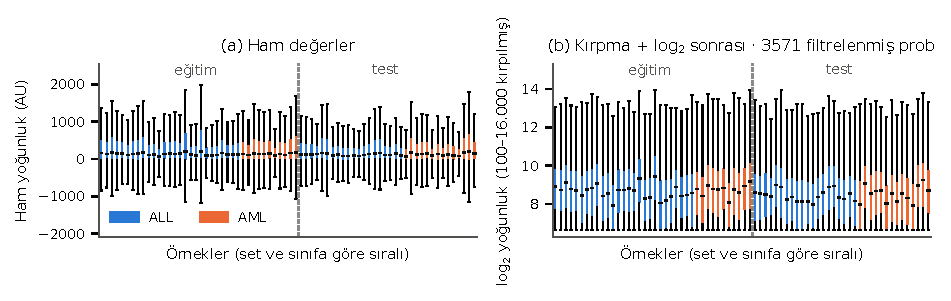
\includegraphics[width=\textwidth]{golub_distributions.pdf}
\caption{Golub örnek dağılımları: (a) ham ortalama fark değerleri, (b) kırpma ve log$_2$ sonrası (\GfiltAllTR{} prob). Kesikli çizgi eğitim/test sınırıdır.}
\label{fig:dist}
\end{figure*}

\subsection{Golub: Boyut İndirgeme ve Ayırt Edici Genler}
PCA'da ilk iki bileşenin açıkladığı varyans sırasıyla \%\GpcATR{} ve \%\GpcBTR{} kadardır; \%80 varyans için \GpcEightyTR{} bileşen gerekir (Şekil~\ref{fig:pca}). \textbf{PC1 sınıfla değil} (Mann--Whitney $p=\GpcAclassTR$), \textbf{eğitim/test ayrımıyla ilişkilidir} ($p=\GpcAsetTR$); sınıf ayrımı PC2'dedir ($p=\GpcBclassTR$). UMAP ALL ve AML'yi büyük ölçüde ayrı kümelerde gösterir. Eğitim setinde Welch $t$ ve Mann--Whitney testleri (Benjamini--Hochberg) ile FDR$<$0,05 düzeyinde \GdeFiveTR{} gen anlamlıdır (AML'de yüksek: \GdeUpAMLTR{}, ALL'de yüksek: \GdeUpALLTR{}). En anlamlı genler (Zyxin, FAH, LEPR, LTC4S, TCF3, HOXA9, CST3) Golub ve ark.'nın bilgi verici genleriyle örtüşür. En iyi 50 genin ısı haritası ve hiyerarşik kümelemesi (Şekil~\ref{fig:heat}) örnekleri iki ana kümeye ayırır; yalnızca \GmisNTR{} ALL örneği (\GmisClust; 67 numara PB kaynaklı tek T-ALL test örneği) AML kümesine düşer. Bu 50 genin testte aynı yönde değişme oranı \%\GsignAgreeTR{}, testte de $p<0{,}05$ olanların sayısı \GtopTestTR{} olarak bulunmuştur.

\begin{figure*}[!t]
\centering
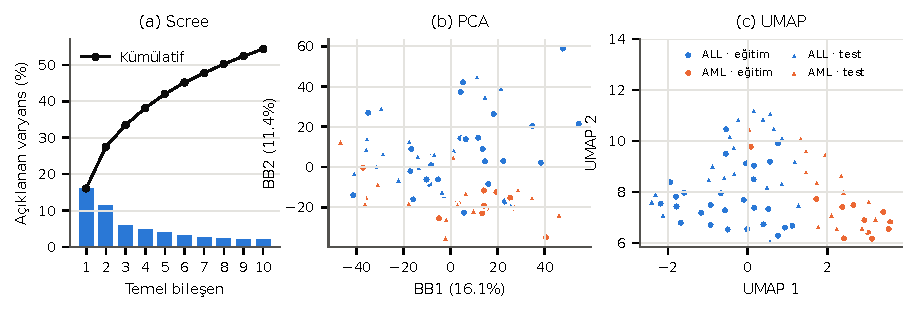
\includegraphics[width=\textwidth]{golub_pca_umap.pdf}
\caption{Golub: (a) PCA açıklanan varyans, (b) PC1--PC2, (c) UMAP (renk: sınıf, işaret: set).}
\label{fig:pca}
\end{figure*}

\begin{figure*}[!t]
\centering
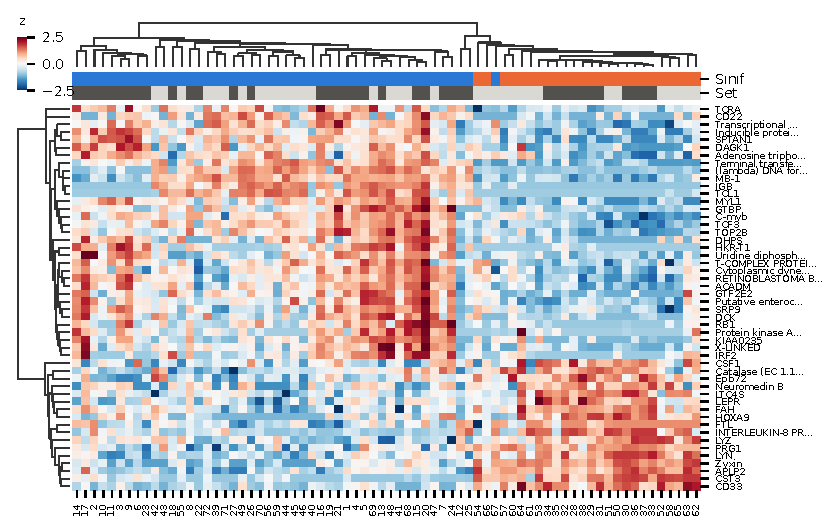
\includegraphics[width=0.84\textwidth]{golub_heatmap_top50.pdf}
\caption{Eğitimde seçilen en iyi 50 genin 72 örnekte z-skor ısı haritası ve hiyerarşik kümelemesi (korelasyon uzaklığı). Şeritler: sınıf; set (koyu: eğitim).}
\label{fig:heat}
\end{figure*}

\subsection{Golub: Eğitim ve Bağımsız Test Setlerinin Karşılaştırılması}\label{sec:batch}
Meta veriye göre \textbf{eğitimdeki 27 ALL'ın tamamı DFCI'dan, 11 AML'nin tamamı CALGB'den gelir ve hepsi kemik iliğidir}; eğitimde sınıf ile merkez tamamen karışıktır, yani bir model sınıf yerine merkez imzasını öğrenebilir. Test seti \GtePBTR{} PB örneği ile St.~Jude ve CCG örnekleri içerir. Örnek başına medyan log$_2$ ifade setler arasında farklıdır ($p=\GmedSetPTR$; Şekil~\ref{fig:batch}a); 58 AFFX kontrol probundan \GaffxTR{} tanesi setler arasında $p<0{,}05$ ile değişir. Sınıf içi Kolmogorov--Smirnov testlerinde ALL'da \GksALLTR{} gen FDR$<$0,05 düzeyinde set farkı gösterirken AML'de hiç gen göstermez. Buna karşın sınıf sinyali korunur: eğitim ve test log$_2$ kat değişimlerinin korelasyonu $r=\GlfcRTR$ düzeyindedir (Şekil~\ref{fig:batch}d). Tek 38/34 bölmenin sonucu bu nedenle merkez ve doku kaymasını da içerecektir.

\begin{figure*}[!t]
\centering
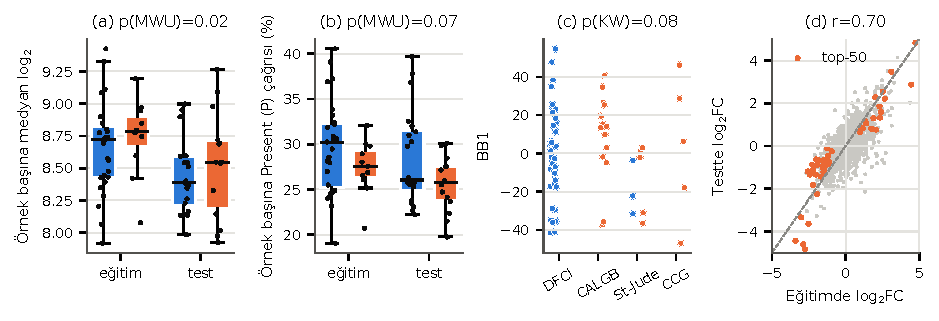
\includegraphics[width=\textwidth]{golub_batch.pdf}
\caption{Golub eğitim/test: (a) örnek medyanı, (b) P çağrısı oranı, (c) merkezlere göre PC1, (d) eğitim ve test log$_2$ kat değişimleri (turuncu: en iyi 50 gen).}
\label{fig:batch}
\end{figure*}

\subsection{GSE13159: Veri Kalitesi, Dağılımlar ve Boyut İndirgeme}
\textbf{Kalite:} \SaffxDropTR{} AFFX kontrol probunun değerleri GEO kaydında tamamen boştur ve çıkarılmıştır; başka eksik değer yoktur. Değerler 0--1 aralığındadır ve her örneğin sıralı değerleri neredeyse aynıdır (en büyük fark \SsortDiffTR{}); bu, kantil normalizasyonun sonucudur. Değerler Beta(1,2;\,3) kantilleriyle örtüşür (medyan \SbetaMedTR{}); yani hedef olarak kuramsal bir 0--1 dağılımı kullanılmıştır. Bu nedenle örnek bazında medyan/IQR karşılaştırması bilgi taşımaz ve Golub'daki kırpma/log dönüşümü uygulanmaz. Örnekler arası ortalama korelasyona IQR kuralı uygulandığında \SoutCorTR{} örnek alt sınırın altında kalmıştır (Şekil~\ref{fig:gse}d); bunlar işaretlenmiş, EDA'da çıkarılmamıştır.
\textbf{Sınıf ve doku:} ALL \%\SallPctTR{}, AML \%\SamlPctTR{} oranındadır. PB örnekleri sınıflara dengeli dağılmıştır (ALL: \SpbALLTR{}, AML: \SpbAMLTR{}); dolayısıyla doku Golub'daki gibi sınıfla karışmaz. Yine de en değişken 5.000 probun ALL içinde \StisALLTR{}, AML içinde \StisAMLTR{} tanesi BM ile PB arasında farklıdır (FDR$<$0,05).
\textbf{Boyut indirgeme:} PC1 varyansın \%\SpcATR{} kadarını açıklar ve doğrudan sınıfı taşır ($p<10^{-300}$); UMAP B-ALL, T-ALL ve AML'yi ayrı kümelerde gösterir (Şekil~\ref{fig:gse}). Büyük örneklemde \SdeFiveTR{} prob FDR$<$0,05 düzeyinde anlamlıdır; bu ölçekte $p$-değerinden çok etki büyüklüğü belirleyicidir. $|t|$ sırasıyla seçilen en iyi 30 genin ısı haritasında (depoda \texttt{gse\_heatmap\_top30}) lenfoid (CD79A, EBF1, DNTT, RAG1) ve miyeloid (KIT, CST3, CFD, MGST1) genler sınıfları ayırır; hiyerarşik kümeleme örneklerin \%\SheatAgreeTR{}'ünü kendi sınıfıyla gruplar.

\begin{figure*}[!t]
\centering
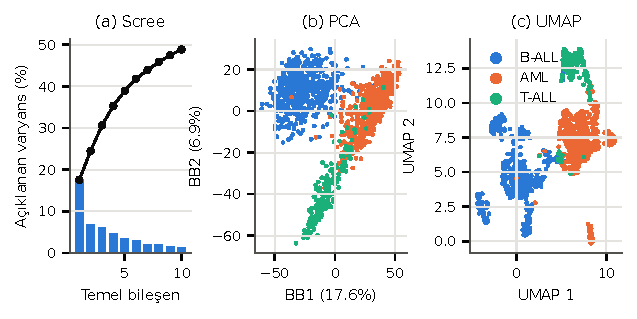
\includegraphics[width=0.665\textwidth]{gse_pca_umap.pdf}\hfill
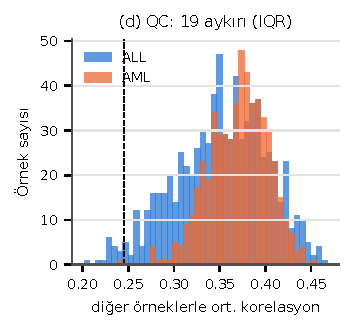
\includegraphics[width=0.325\textwidth]{gse_qc_corr.pdf}
\caption{GSE13159: (a) açıklanan varyans, (b) PCA, (c) UMAP (en değişken 5.000 prob), (d) korelasyon tabanlı kalite kontrolü (kesikli: IQR alt sınırı).}
\label{fig:gse}
\end{figure*}

\subsection{İki Veri Seti Arasındaki Dağılım Farkları}\label{sec:cross}
Ortak genlerde iki veri setinin ölçekleri tamamen farklıdır (Golub log$_2$ medyanı \SmedGTR{}, GSE13159 medyanı \SmedSTR{}); ham değerlerle yapılan ortak PCA'da PC1 varyansın \%\SrawPConeTR{}'unu açıklar ve yalnızca veri setini ayırır (Şekil~\ref{fig:cross}b). Her veri seti kendi içinde standartlaştırıldığında veri seti ayrımı kaybolur, sınıf yapısı ortaklaşır (Şekil~\ref{fig:cross}c). Gen ortalamalarının sıralaması iki platformda orta düzeyde uyumludur ($\rho=\SmeanRhoTR$). Sınıf etkileri tutarlıdır: AML/ALL farklarının korelasyonu $r=\SlfcRTR$ düzeyindedir ve iki veri setinin en iyi 100 geninden \SovHundTR{} tanesi ortaktır (şans beklentisi \SovHundExpTR{}, hipergeometrik $p=\SovHundPTR$). Ortak genler lenfoid (CD19, CD22, CD79A, DNTT, VPREB1) ve miyeloid (CD33, CST3, ZYX, LYN) belirteçleri içerir.

\begin{figure*}[!t]
\centering
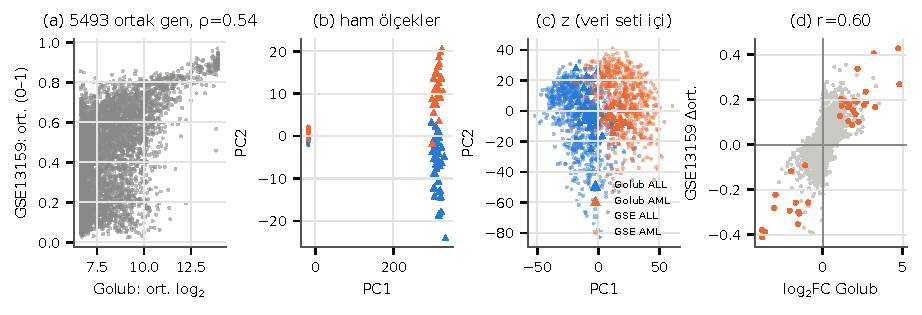
\includegraphics[width=\textwidth]{cross_dataset.pdf}
\caption{Golub ve GSE13159 (\ScommonGTR{} ortak gen): (a) gen ortalamaları, (b) ham ölçeklerle ve (c) veri seti içi z-skorla ortak PCA, (d) AML/ALL farkları (turuncu: ortak en iyi genler).}
\label{fig:cross}
\end{figure*}

\subsection{Bulguların Numaralı Özeti ve Modelleme İçin Çıkarımlar}
\begin{enumerate}[label=\textbf{B\arabic*.}]
\item Etiketler hasta numarasıyla eşlenmeli; sütun sırasıyla eşleme \GmisPosTR{} örneği yanlış etiketler.
\item INF bir ön işleme ürünüdür; doldurmak yerine katlar içinde kırpma + log$_2$ uygulanmalıdır.
\item Değerlerin yaklaşık yarısı (\%\GbelowClipTR{}) 100'ün altındadır, sınıf sinyali ise az sayıda gende yoğundur; ifade filtresi ve gen sayısı ($k$) seçimi eğitim katlarında yapılmalıdır.
\item Golub eğitiminde sınıf ile merkez çakışır; tek 38/34 sonucu iç içe CV ile birlikte yorumlanmalıdır.
\item Sınıflar dengesizdir; tabakalı bölme, \texttt{class\_weight} ve dengeli doğruluk gereklidir.
\item İki platformun ölçekleri farklıdır; aktarım ancak ortak genlerde veri seti içi standardizasyonla anlamlıdır.
\item GSE13159'da doku tipi ve korelasyon aykırıları duyarlılık analizinde dikkate alınmalıdır.
\end{enumerate}

%======================================================================
\section{FİNALE KADAR PLAN}
\textbf{Yöntemler ve gerekçe:} (1) \emph{LASSO/elastik ağ düzenlileştirmeli lojistik regresyon}: gömülü gen seçimi, ilişkili genleri birlikte tutma ve yorumlanabilir katsayılar~\cite{zou2005}; (2) \emph{doğrusal SVM}: mikrodizi verisinde tutarlı başarı~\cite{furey2000,statnikov2008}, katlar içinde filtreyle; (3) \emph{rastgele orman}: doğrusal olmayan etkileşimler, ölçeklemeye duyarsızlık ve özellik önemi~\cite{diaz2006}. \textbf{Hedeflenen bonuslar:} B1 (dropout'lu MLP), B2 (katlar içinde $\le$500 genle TabPFN~\cite{hollmann2025}). \textbf{Takvim (hafta):} 1--2 pipeline ve 38/34; 3--4 iç içe CV ve istatistiksel karşılaştırma; 5 GSE13159 ve aktarım; 6 bonuslar; 7--8 yorumlanabilirlik, rapor, video. \textbf{Riskler (önlem):} küçük $n$ (tekrarlı CV, güven aralığı), merkez/doku karışıklığı (duyarlılık analizi), platform farkı (veri seti içi standardizasyon), aşırı öğrenme (erken durdurma).

%======================================================================
\section{GENAI KULLANIM BEYANI VE ÖZGÜNLÜK}
\begin{table}[!h]
\centering\scriptsize\setlength{\tabcolsep}{2pt}
\begin{tabularx}{\columnwidth}{@{}p{1.5cm}p{1.9cm}X X@{}}
\toprule
\textbf{Araç / sürüm} & \textbf{Amaç; bölüm/dosya} & \textbf{Öğrencinin değişikliği} & \textbf{Doğrulama}\\
\midrule
Claude Opus 5.5 (Anthropic), 08.11.2026 & Literatür sorguları, DOI kontrolü; Bölüm II & Kapsamı yönerge isterleriyle sınırladı; 6 sayfa için tabloyu kısalttırdı & DOI'ler Crossref kayıtlarıyla eşlendi\\
Claude Opus 5.5 & EDA kodu; \texttt{src/*.py} & GSE13159'u seçti, GEO verisini kendisi indirdi; alt tip, doku ve 0--1 ölçek kararlarını verdi & Kod yeniden çalıştırıldı; 3571/3051 gen sayıları literatürle tuttu\\
Claude Opus 5.5 & Rapor metni, LaTeX & İstenmeyen içeriği çıkarttı; Kaggle lisansını (CC0) kontrol etti & Sayılar \texttt{results/} çıktılarından otomatik basıldı\\
\bottomrule
\end{tabularx}
\end{table}
İstem özetleri ve ayrıntılı beyan: depoda \texttt{docs/GenAI\_kullanim\_beyani.md}. Tüm kod ve yorumlar öğrenci tarafından gözden geçirilmiştir.

\section*{TEŞEKKÜR}
Claude Opus 5.5 (Anthropic) yardımcı araç olarak kullanılmıştır (Bölüm VI); sorumluluk yazara aittir.

\bibliographystyle{IEEEtran}
{\footnotesize\bibliography{../references_doi}}

\end{document}
